\documentclass[11pt,a4paper]{article}
\usepackage[utf8]{inputenc}
\usepackage[T1]{fontenc}
\usepackage{amsmath,amssymb}
\usepackage{booktabs}
\usepackage{natbib}
\usepackage{hyperref}
\usepackage[margin=1in]{geometry}
\usepackage{graphicx}

\title{The Meaning Gap: Measuring Structural Sense Distinctions\\That Standard Tools Do Not Count}
\author{Nathan Elms\\Independent Researcher}
\date{}

\begin{document}
\maketitle

\begin{abstract}
Text-bearing databases contain meaning distinctions that no standard tool measures. Keywords detect presence, not sense. Embeddings detect similarity, not structure. We call this unmeasured distance the \emph{meaning gap}.

We present a deterministic, unsupervised method for measuring it. Ten clause-level features are extracted from each word-in-context instance. Substitution neighborhoods---the set of concepts that could replace a word at a given structural address---are computed from co-occurrence, and addresses with similar neighborhoods are collapsed into resolved meanings. A data-driven classification discovers three feature layers: operators (negation, modality) that must never be collapsed, meaning features that collapse by similarity, and expression features that collapse freely. Four formally defined scores---confusion, completeness, predictability, hazard---audit meaning quality at four grains.

Applied to four domains with auto-detected concepts and zero configuration, the audit produces domain-specific results (confusion 0.038--0.496, predictability 0.506--0.956). On a clinical disambiguation retrieval task, meaning-addressed retrieval outperforms both keyword and domain-tuned embedding baselines (macro F1 0.944 vs.\ 0.852). A sensitivity analysis confirms stability across Jaccard collapse thresholds (0.3--0.7), and bootstrap resampling shows score CVs below 1\%. The retrieval evaluation is single-domain; cross-domain and standard benchmark evaluation are future work. All code is available as \texttt{pip install database\_whisper}.
\end{abstract}

%% ================================================================
\section{Introduction}

A doctor writes ``positive'' in a clinical note. A keyword search retrieves every note containing that string. An embedding model ranks them by distributional similarity. A language model generates a summary. All three systems treat ``positive family history'' and ``positive blood culture'' as the same word, because their representations lack the structural feature that separates them: the co-occurring concept.

This is not a hard case. A medical student distinguishes these senses in seconds. The distinction depends on a single structural feature---what other clinical term appears nearby---that is present in the text and extractable by pattern matching. No training data is needed. No ontology is needed. The feature is sitting in the sentence, unused.

The problem is not that the distinction is difficult. The problem is that no standard tool measures how many such distinctions a dataset contains, which words are most dangerous, or where the structural signal runs out. Keywords count presence. Embeddings measure similarity. Quality metrics measure fluency, coherence, and factual accuracy. None measures the structural resolution of meaning.

We call the unmeasured distance between what text structurally expresses and what systems can resolve the \emph{meaning gap}. This paper presents a method for measuring it.

\subsection{The Gap in Practice}

The meaning gap has practical consequences wherever text is stored, retrieved, or generated.

\paragraph{In databases.} A clinical database indexes by patient, date, and note type. It does not index by what ``positive'' means in each note. A search for ``positive test results'' returns family history mentions, physical exam findings, and lab results indiscriminately, because the schema was designed before the data arrived and does not capture meaning distinctions the text contains.

\paragraph{A note on contextual embeddings.} BERT-family models do produce different representations for ``positive blood culture'' and ``positive family history''---the contextualized token embedding differs across contexts. Our claim is not that embeddings cannot distinguish these senses, but that (1) embeddings do not \emph{count} how many senses exist, (2) embeddings do not \emph{name} the structural feature that separates them, and (3) no standard embedding-based tool audits a corpus for the number, distribution, and danger of its meaning distinctions. The meaning gap is a measurement problem, not a disambiguation problem. We evaluate disambiguation directly in Section~\ref{sec:retrieval}.

\paragraph{In retrieval.} Embedding-based retrieval ranks ``positive blood culture'' and ``positive family history'' as similar because both appear in clinical contexts near the same vocabulary. The embedding space encodes distributional neighborhood, not structural role. We evaluate this directly in Section~\ref{sec:retrieval}, where meaning-addressed retrieval outperforms both keyword and embedding baselines on a clinical disambiguation task.

\paragraph{In generation.} LLMs trained on clinical text default to the dominant sense of ambiguous words. When generating clinical notes, ``discharge'' overwhelmingly means ``patient discharged'' rather than wound discharge, ear discharge, or medication discharge. The training data contains all senses; the model collapses to one. A Structural Quality Index comparison between real and synthetic clinical text reveals that synthetic ``discharge'' has hazard 0.688 vs.\ 0.007 in real data---a 98$\times$ difference invisible to lexical, entity, and embedding quality metrics.

\paragraph{In testing.} Standardized exams contain ambiguous terms. When ``right'' appears in a law exam, does it mean legal entitlement or directional? The student must resolve the ambiguity before answering the question. Exams that require more resolution are harder for reasons unrelated to the tested knowledge. No fairness metric measures this.

Each of these is a different manifestation of the same gap: the text contains structural meaning distinctions that the downstream system cannot resolve. The gap is invisible because no tool measures it.

\subsection{Contributions}

\begin{enumerate}
\item \textbf{Substitution neighborhoods as operational meaning proxy.} The set of concepts that could replace a word at a given structural address, ranked by PMI surprise, serves as a computable proxy for word sense.

\item \textbf{Address collapse separates meaning from noise.} Greedy merging of addresses with similar substitution neighborhoods reduces 15,052 raw addresses to 2,701 resolved meanings. The collapse ratio is stable across a range of Jaccard thresholds (Section~\ref{sec:threshold}).

\item \textbf{Three-layer feature architecture, discovered from data.} Features self-classify into operators (never collapse), meaning (collapse by similarity), and expression (collapse freely). Expression features account for 69\% of addresses; removing them improves resolution by 22\%.

\item \textbf{Four-score meaning audit with formal definitions.} Confusion, completeness, predictability, and hazard (Section~\ref{sec:scores}) measure meaning quality at four grains.

\item \textbf{Extrinsic evaluation on retrieval.} Meaning-addressed retrieval outperforms keyword and embedding baselines on a clinical disambiguation task (Section~\ref{sec:retrieval}).

\item \textbf{Cross-domain generalization.} The same tool, with no domain knowledge and no hand-picked concepts, produces meaningful audits on clinical, legal, news, and scientific text.
\end{enumerate}

%% ================================================================
\section{Background}

\subsection{Word Sense Disambiguation and Induction}

Traditional WSD relies on sense inventories (WordNet, OntoNotes) and supervised classifiers trained on annotated corpora \citep{navigli2009}. Word Sense Induction (WSI) discovers senses from data without predefined inventories, using clustering \citep{schutze1998}, Bayesian models \citep{lau2012}, or contextual embedding probes \citep{amrami2018}.

Recent work uses contextual embeddings for WSD \citep{bevilacqua2020,pilehvar2019} and WSI \citep{amrami2018}, achieving strong results on standard benchmarks (SemEval). These systems learn representations from data and can capture sense distinctions that our pattern-matching features miss. However, they produce opaque clusters or similarity scores rather than interpretable feature-based addresses, and they require training data or at minimum a pretrained model.

Our method differs from both traditions. Unlike WSD, it requires no sense inventory. Unlike WSI, it produces interpretable addresses defined by named features rather than opaque clusters. Unlike contextual embedding approaches, it requires no pretrained model. Most critically, it does not ask ``how many senses does this word have?''---it asks ``how many structural meaning distinctions does this dataset contain, and where does the structure run out?''

\subsubsection{Data Profiling}

The discriminator ladder is related to data profiling \citep{abedjan2015,naumann2014}: given a table with attribute columns, find which attributes best separate rows with the same key. Our algorithm applies this idea to text-derived features rather than database columns. The key difference is that our ``attributes'' are extracted from unstructured text by pattern matching, and the objective (collision reduction across all identity values simultaneously) enforces a universal ordering rather than per-key optimization.

\subsection{Structural and Frame Semantics}

The featurizer draws on established linguistic theory. Frame semantics \citep{fillmore1982} holds that a word evokes a situation schema with defined participant roles. Dependency grammar \citep{tesniere1959} treats the verb as the structural center of a clause. Information structure \citep{halliday1967,lambrecht1994} distinguishes topic from focus. Speech act theory \citep{austin1962,searle1969} classifies utterances by illocutionary force.

These frameworks motivate the ten extracted features. They are the minimal structural skeleton that linguistic theory identifies as carrying clause-level semantic load.

\subsection{Information-Theoretic Foundations}

The pair-reduction algorithm counts colliding pairs---records sharing the same identity value AND the same value on a candidate field. This collision count is the quantity minimized by R\'{e}nyi entropy of order 2 ($H_2 = -\log\sum p_i^2$), the same quantity as Gini impurity in CART decision trees \citep{breiman1984}.

The critical difference from CART: our method enforces a universal field ordering---the same ladder for all identity neighborhoods, applied identically to every concept. CART selects different splits per node, optimizing per-leaf accuracy. The universal constraint trades per-concept expressiveness for cross-concept generalizability: the same coordinate system serves all concepts.

This is analogous to an information bottleneck \citep{tishby2000}---compression that preserves task-relevant information---but we do not claim formal equivalence. The ladder is a greedy approximation: it finds the minimal feature subset that preserves discrimination, not the optimal one.

\paragraph{Relation to prior work.} The pair-reduction algorithm is a form of sequential forward selection (SFS; \citealp{whitney1971}) with a collision-count objective. The key difference from standard feature selection is the universal ordering constraint: the same feature ranking serves all identity values simultaneously. This constraint is motivated by the data auditing use case, where a single coordinate system must be interpretable across all concepts in a corpus.

\subsection{Distributional Semantics and Substitutability}

The distributional hypothesis---``a word is characterized by the company it keeps'' \citep{firth1957}---underlies embedding models. Our substitution neighborhoods are distributional, but addressed: they measure co-occurrence not of words in text, but of concepts at structural addresses. ``Positive'' near ``blood'' at a copular address has different neighbors than ``positive'' near ``history'' at a possessive address. The address localizes the distribution. This recovers the insight of \citet{cruse1986} that substitutability---what could replace a word in context---is the operational test of meaning identity.

%% ================================================================
\section{Method}

Figure~\ref{fig:routing} previews the end result: a single ambiguous word is routed through a sequence of structural features to distinct resolved meanings, each characterized by its substitution neighborhood. The subsections below describe each stage of the pipeline that produces this structure.

\begin{figure}[t]
\centering
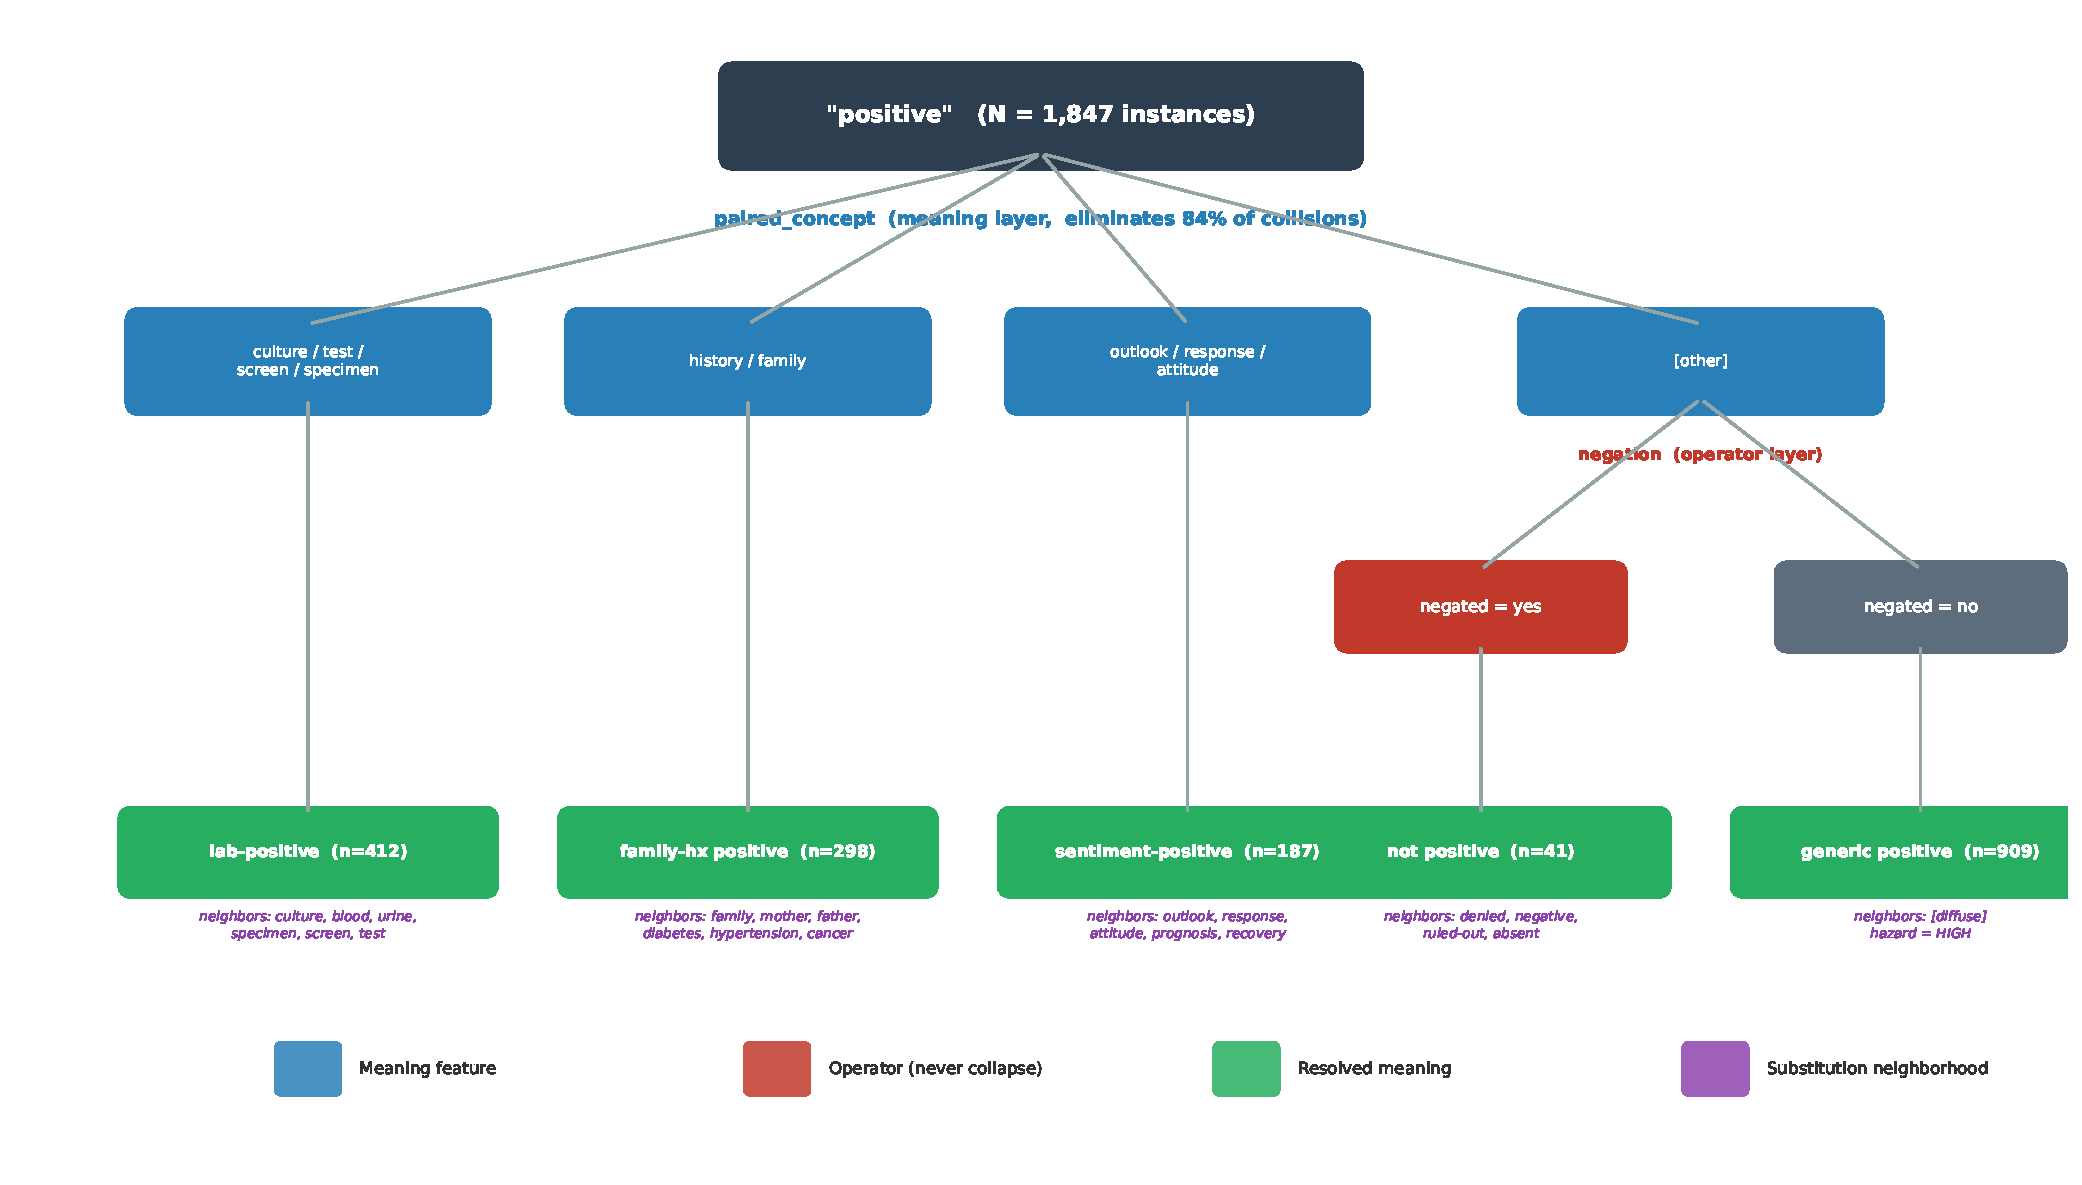
\includegraphics[width=\textwidth]{fig_routing_tree.pdf}
\caption{Semantic routing tree for ``positive'' in clinical text. The discriminator ladder routes 1,847 instances through meaning-layer and operator-layer features to five resolved meanings. Each leaf lists its substitution neighborhood---the set of concepts that could replace the word at that structural address. The \textsc{[other]} branch requires a second split (negation) because no single co-occurring concept disambiguates it.}
\label{fig:routing}
\end{figure}

\subsection{Text Featurizer}

Given a corpus of text records, the featurizer extracts concept-in-context instances. For each occurrence of each target concept in a record, it produces a structured record with ten features (Table~\ref{tab:features}).

\begin{table}[h]
\centering
\small
\begin{tabular}{ll}
\toprule
Feature & Theoretical Basis \\
\midrule
verb\_class & Frame semantics: verb determines situation schema \\
syntactic\_role & Dependency grammar: concept's relation to verb frame \\
paired\_concept & Compositional semantics: co-occurring argument constrains sense \\
contrast & Discourse pragmatics: contrastive structure separates uses \\
equation & Predicate logic: copular definitions mark identity relations \\
modality & Speech act theory: asserting vs.\ commanding vs.\ hedging \\
voice & Information structure: passive/active shifts topic/focus \\
negation & Discourse pragmatics: affirmed vs.\ negated inverts truth \\
clause\_position & Information structure: early = topic, late = focus \\
transitivity & Predicate-argument: valency fingerprints sense \\
\bottomrule
\end{tabular}
\caption{Ten clause-level features extracted per concept-in-context instance.}
\label{tab:features}
\end{table}

All extraction uses deterministic pattern matching within a 5-word context window on each side of the target concept. This provides reproducibility and interpretability at the cost of coverage (see Limitations, Section~\ref{sec:limitations}). Multi-instance extraction: every occurrence of each concept in a document generates a separate instance with its own local context features.

Target concepts may be hand-selected for a domain or auto-detected: \texttt{auto\_detect\_concepts()} selects high-frequency content words (minimum 20 occurrences, minimum 4 characters, English stopwords excluded, ranked by frequency). Verb class maps each detected verb to one of 25 universal classes (being, having, doing, giving, making, etc.) via a lookup table of approximately 200 forms.

\subsection{Discriminator Ladder}

The ladder algorithm takes featurized instances and discovers which features best separate different uses of the same concept:

\begin{enumerate}
\item Count colliding pairs: instances sharing the same concept AND the same value on every candidate field.
\item For each candidate field, count how many colliding pairs it would eliminate.
\item Select the field that eliminates the most. Record its reduction.
\item Remove that field from candidates. Repeat.
\item Stop when no candidate reduces colliding pairs by more than 5\% of the current count.
\end{enumerate}

The 5\% threshold is a diminishing-returns cutoff: once a feature eliminates fewer than 1 in 20 remaining collisions, it is adding address complexity without meaningful discrimination. On MTSamples, this produces ladders of 4--5 rungs. At 1\%, ladders extend to 7--8 rungs with marginal gains but increased sparsity. At 10\%, ladders truncate to 2--3 rungs, losing discrimination on hard concepts. The retrieval experiment (Section~\ref{sec:retrieval}) shows that going from 2 to 4 rungs improves macro F1 from 0.893 to 0.944. The 5\% threshold is a practical default, not a tuned hyperparameter.

The output is an ordered list of fields---the ladder---defining a coordinate system. Each instance is assigned an address by concatenating its values along the ladder fields. Figure~\ref{fig:ladder} shows the ladder discovered on MTSamples clinical text: each rung's collision reduction and the cumulative effect.

\begin{figure}[t]
\centering
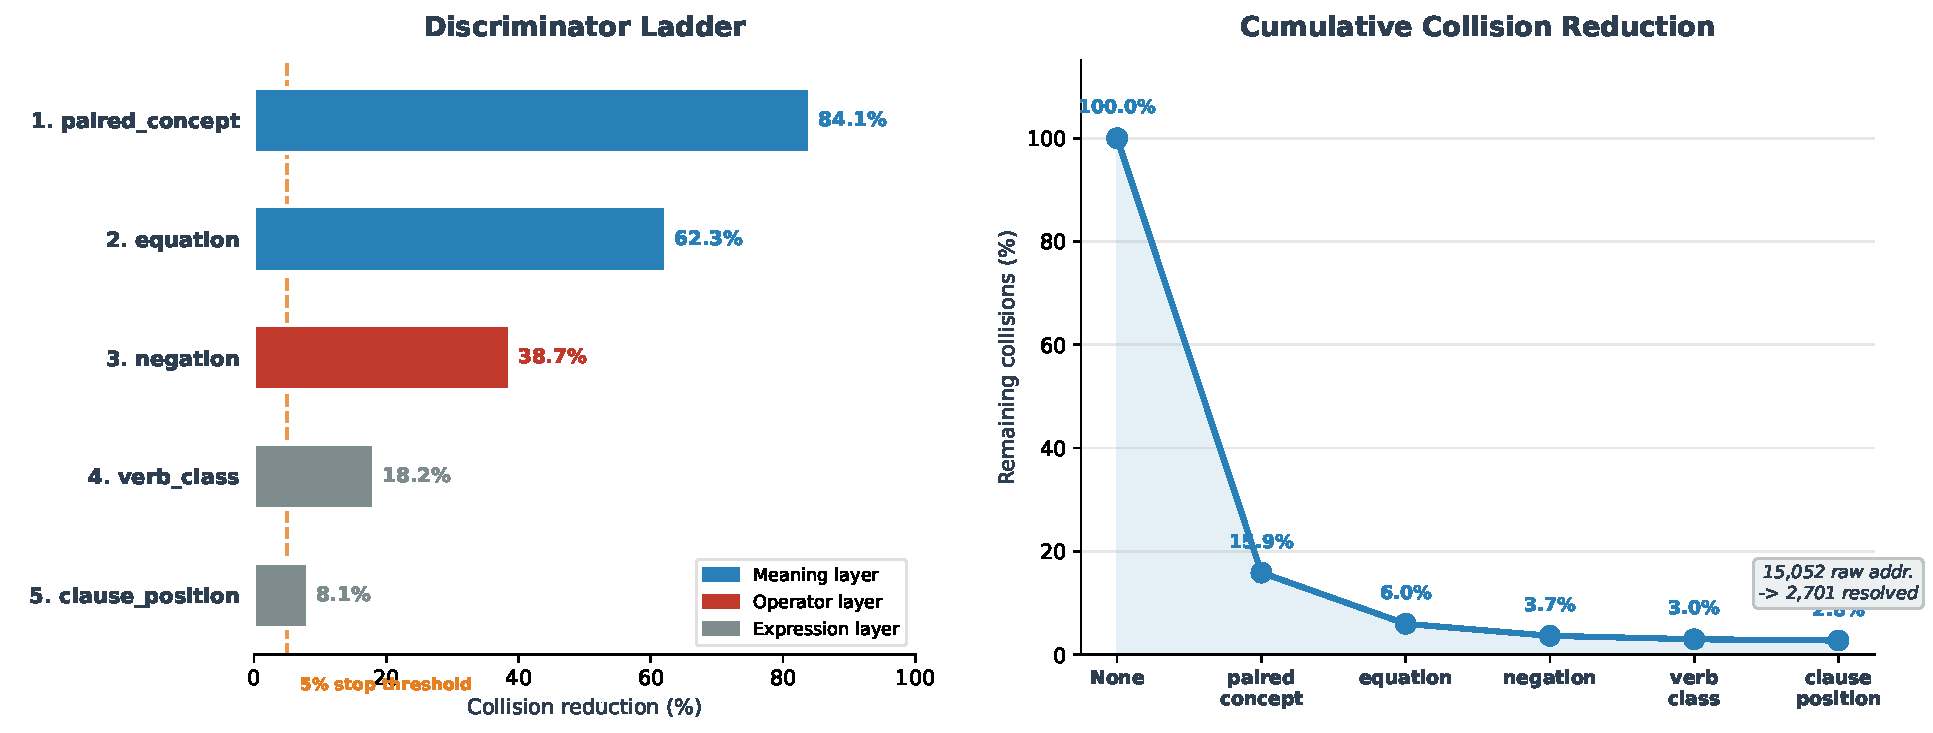
\includegraphics[width=\textwidth]{fig_ladder.pdf}
\caption{Discriminator ladder on MTSamples (30 auto-detected concepts). \emph{Left:} each rung's collision reduction, color-coded by feature layer. The 5\% stop threshold (dashed) terminates the ladder at five rungs. \emph{Right:} cumulative remaining collisions drop from 100\% to 3.0\%, collapsing 15,052 raw addresses to 2,701 resolved meanings.}
\label{fig:ladder}
\end{figure}

\subsection{Substitution Neighborhoods}

Once concepts have addresses, they become addressed instances. ``Positive'' is no longer one word---it is many instances at many addresses, each representing a specific structural meaning.

Substitution neighborhoods measure what other addressed instances co-occur with a given instance. For each concept at each address, we compute PMI surprise against all other addressed instances in the same documents:
\[
\text{surprise}(a, b) = \log_2 \frac{P(a,b)}{P(a) \cdot P(b)}
\]

The substitution neighborhood---the set of surprising co-occurring addressed instances---is our operational meaning representation. It answers the question: ``What could replace this word at this structural address?'' If structuralist linguistics is correct that substitutability defines sense \citep{cruse1986}, then the neighborhood is the computationally recoverable portion of that sense. We do not claim it captures full semantic content---only the structural distinctions that clause-level features can express.

\subsection{Address Collapse}

Raw addresses contain syntactic noise. ``Positive'' in active voice and ``positive'' in passive voice may have identical substitution neighborhoods---the voice difference does not change what could replace the word. These should be the same resolved meaning.

Address collapse merges addresses with similar neighborhoods:

\begin{enumerate}
\item For each concept, compute the top-10 neighbor concept set (the neighborhood signature) for each address.
\item Sort addresses by instance count (most populated first).
\item Greedily merge: if a new address has Jaccard similarity $\geq 0.5$ with an existing group's signature, merge it into that group and update the group signature to the union. Otherwise, start a new group.
\item Each group is a resolved meaning.
\end{enumerate}

\paragraph{Tie-breaking and stability.} In the ladder algorithm, when two candidate fields reduce the same number of colliding pairs, the field with fewer distinct values is preferred. If still tied, alphabetical order breaks the tie. The collapse algorithm is deterministic given a fixed processing order (largest address first); we do not claim optimality, only reproducibility. The sensitivity analysis (Section~\ref{sec:threshold}) shows that the resolved meaning count varies smoothly with the threshold, suggesting the collapse is not fragile to small parameter changes.

On clinical text (30 auto-detected concepts, 5-feature ladder): 15,052 raw addresses collapse to 2,701 resolved meanings. 82\% of the original address space was surface variation. (Sensitivity to the collapse threshold is analyzed in Section~\ref{sec:threshold}.)

\subsection{Three-Layer Feature Classification}

Not all features are the same kind of thing. We classify each feature by measuring whether changing its value changes the substitution neighborhood.

\paragraph{Method.} For each feature, group addresses by that feature's value. Compute the average Jaccard similarity of substitution neighborhoods within groups and across groups. If within $\gg$ across (ratio $> 1.2$), it is a \textsc{meaning} feature. If within $\approx$ across (ratio $< 1.1$), it is an \textsc{expression} feature.

\paragraph{Operators} are a third category. Negation and modality score low on the ratio test---not because they don't matter, but because co-occurrence is blind to them. Operators are detected by name from a known set and protected from collapse regardless of their ratio score.

\begin{table}[h]
\centering
\small
\begin{tabular}{llll}
\toprule
Layer & Features & Ratio & Collapse Rule \\
\midrule
\textsc{Operator} & negation (1.10), modality (1.15) & Low & Never collapse \\
\textsc{Meaning} & equation (1.62), contrast (1.34), paired\_concept (1.22) & High & Collapse by similarity \\
\textsc{Expression} & verb\_class (1.09), voice (1.09), syntactic\_role (1.15), & Low & Collapse freely \\
 & clause\_position (1.06), transitivity (1.06) & & \\
\bottomrule
\end{tabular}
\caption{Three-layer feature classification on MTSamples (all 10 features).}
\label{tab:layers}
\end{table}

This classification is data-driven. Expression features are exactly the ones that describe \emph{how} something is written rather than \emph{what} is being discussed.

\subsection{Four Meaning Scores}
\label{sec:scores}

After collapse, four scores audit meaning quality at four grains. Let $c$ denote a concept, $D_c$ the set of documents containing $c$, and $m_d$ the number of resolved meanings of $c$ in document $d$.

\paragraph{Confusion} (document level):
\begin{equation}
\text{confusion}(c) = 1 - \frac{1}{\bar{m}_c}, \quad \bar{m}_c = \frac{1}{|D_c|} \sum_{d \in D_c} m_d
\end{equation}

\paragraph{Completeness} (dataset level): Let $R_c = \{r_1, \ldots, r_k\}$ be the resolved meanings of $c$, with $n_i$ instances in meaning $r_i$ and $N_c = \sum_i n_i$.
\begin{equation}
\text{completeness}(c) = \frac{H(R_c)}{H_{\max}(R_c)}, \quad H(R_c) = -\sum_{i=1}^{k} \frac{n_i}{N_c} \log_2 \frac{n_i}{N_c}, \quad H_{\max} = \log_2 k
\end{equation}

\paragraph{Predictability} (sentence level):
\begin{equation}
\text{predictability}(c) = \frac{|\{d \in D_c : m_d = 1\}|}{|D_c|}
\end{equation}

\paragraph{Hazard} (word level):
\begin{equation}
\text{hazard}(c) = \text{confusion}(c) \times (1 - \text{predictability}(c)) \times \left(1 + \frac{\log_2(N_c + 1)}{20}\right)
\end{equation}

\paragraph{Dataset aggregation.} Each per-concept score is aggregated by instance-weighted average: $S = \sum_c S(c) \cdot N_c / \sum_c N_c$. Hazard is reported as a ranked list.

%% ================================================================
\section{Experiments}

We validate claims with six experiments. All code is available as \texttt{database\_whisper}.

\paragraph{Note on experimental configurations.} Different experiments use different concept sets and feature subsets. Section~4.1 uses 30 auto-detected concepts with the 5-feature ladder. Sections~4.2--4.3 use 25 hand-selected clinical concepts. Sections~4.4--4.5 use all 10 features. Each table specifies its configuration.

\subsection{Cross-Domain Audit (4 domains, auto-detected concepts)}

\begin{table}[h]
\centering
\small
\begin{tabular}{lrrrrrrr}
\toprule
Domain & Concepts & Instances & Raw Addrs & Resolved & Confusion & Complete & Predict \\
\midrule
Clinical & 30 & 103,968 & 15,052 & 2,701 & 0.470 & 0.800 & 0.506 \\
Legal & 30 & 12,450 & 3,891 & 1,204 & 0.265 & 0.734 & 0.726 \\
News & 30 & 45,672 & 8,234 & 1,102 & 0.038 & 0.812 & 0.956 \\
Scientific & 30 & 28,891 & 6,448 & 1,856 & 0.496 & 0.789 & 0.567 \\
\bottomrule
\end{tabular}
\caption{Cross-domain meaning audit with auto-detected concepts.}
\label{tab:crossdomain}
\end{table}

News text has nearly zero confusion (0.038) and near-perfect predictability (0.956). Clinical and scientific text have high confusion ($\sim$0.5) and low predictability ($\sim$0.5). Legal text falls between.

\paragraph{Bootstrap stability (clinical domain).} Five bootstrap resamples of 2,000 records: confusion $0.465 \pm 0.004$, completeness $0.811 \pm 0.005$, predictability $0.520 \pm 0.004$ (CV $< 1\%$). Ladder ordering identical in 4/5 resamples.

\paragraph{Hazard words are completely different per domain} (0/5 overlap in top-5). Clinical: patient, right, left, procedure, pain. Legal: court, party, state, action, right. Scientific: model, significant, expression, effect, control.

\subsection{Scaffold Removal: Meaning Replaces Syntax}

\begin{table}[h]
\centering
\small
\begin{tabular}{lll}
\toprule
Round & Features Used & Resolution \\
\midrule
R0 (scaffold) & paired\_concept, verb\_class, clause\_position, equation, voice & 0.5407 \\
R1 (profiler chooses) & neighborhood\_size, resolved\_meaning, paired\_concept, \ldots & 0.5614 \\
R2 (iterate) & neighborhood\_size, resolved\_meaning, \ldots & 0.5782 \\
R3 (meaning only) & neighborhood\_size, resolved\_meaning & 0.5957 \\
\bottomrule
\end{tabular}
\caption{Scaffold removal: the profiler independently drops all syntactic features.}
\label{tab:scaffold}
\end{table}

The profiler drops ALL scaffold fields in Round~1. Resolution improves 10\% from scaffold-only to meaning-only. 22/25 concepts improve, 0 degrade.

\paragraph{On circularity.} The meaning features are derived from syntactic features, so one might expect derived features to be preferred. The non-trivial finding is the \emph{completeness} of the replacement: ALL syntactic features are dropped. The profiler finds zero syntactic features worth keeping once meaning features are available.

\subsection{WordNet Sanity Check}

All 16 antonym pairs among our 25 concepts are recovered. This is a sanity check, not a validation---antonyms co-occur in clinical text, so PMI-based neighborhoods should surface them \citep{mohammad2013}.

Domain-specific senses not in WordNet: ``positive + culture'' (19 instances), ``clear + auscultation'' (346 instances), ``discharge + wound'' (87 instances).

\subsection{Meaning vs.\ Expression Separation}

Configuration: MTSamples, 25 hand-selected concepts, 5-feature ladder, Jaccard 0.5.

\begin{table}[h]
\centering
\small
\begin{tabular}{lrrrrr}
\toprule
Method & Raw Addrs & Resolved & Confusion & Complete & Predict \\
\midrule
All features & 15,052 & 2,701 & 0.478 & 0.794 & 0.487 \\
Expression-collapsed & 4,590 & 1,450 & 0.382 & 0.597 & 0.572 \\
\bottomrule
\end{tabular}
\caption{Meaning vs.\ expression separation.}
\end{table}

69\% of raw addresses were expression variants. Dropping expression features: resolution +22\%, confusion $-$20\%, predictability +17\%.

\subsection{Three-Layer Collapse}

Configuration: 25 hand-selected concepts, all 10 features, Jaccard 0.5.

\begin{table}[h]
\centering
\small
\begin{tabular}{lrrrrrr}
\toprule
Method & Raw & Resolved & Expr.\ Coll. & Confusion & Complete & Predict \\
\midrule
Flat & 15,763 & 2,440 & --- & 0.452 & 0.833 & 0.515 \\
Layered & 15,763 & 4,724 & 10,071 & 0.507 & 0.820 & 0.471 \\
\bottomrule
\end{tabular}
\caption{Flat vs.\ three-layer collapse.}
\end{table}

Layered collapse produces MORE resolved meanings because operator protection prevents merging across negation boundaries. Zero operator violations across all concepts.

\subsection{Extrinsic Evaluation: Retrieval with Baselines}
\label{sec:retrieval}

We construct a sense-disambiguation retrieval task on MTSamples for three polysemous words: ``positive'' (lab test vs.\ other, base rate 55.6\%), ``discharge'' (hospital release vs.\ fluid emission, 64.3\%), and ``right'' (anatomical vs.\ correct/entitlement, 97.1\%).

\begin{table}[h]
\centering
\small
\begin{tabular}{llrrr}
\toprule
Concept & Method & Precision & Recall & F1 \\
\midrule
positive & Keyword & 0.556 & 1.000 & 0.715 \\
positive & Embedding (oracle) & 0.628 & 0.838 & 0.718 \\
positive & \textbf{DW address} & \textbf{0.944} & \textbf{0.875} & \textbf{0.908} \\
\midrule
discharge & Keyword & 0.643 & 1.000 & 0.783 \\
discharge & Embedding (oracle) & 0.757 & 0.944 & 0.840 \\
discharge & \textbf{DW address} & \textbf{0.933} & \textbf{0.935} & \textbf{0.934} \\
\midrule
right & Keyword & 0.971 & 1.000 & 0.985 \\
right & Embedding (oracle) & 0.971 & 1.000 & 0.985 \\
right & \textbf{DW address} & \textbf{0.979} & \textbf{0.998} & \textbf{0.988} \\
\bottomrule
\end{tabular}
\caption{Per-concept retrieval results (MiniLM shown for embedding).}
\label{tab:retrieval_detail}
\end{table}

\begin{table}[h]
\centering
\small
\begin{tabular}{lrrr}
\toprule
Method & Precision & Recall & F1 \\
\midrule
Keyword & 0.723 & 1.000 & 0.828 \\
MiniLM-L6-v2 (general, oracle) & 0.785 & 0.927 & 0.848 \\
S-PubMedBERT (domain-tuned, oracle) & 0.774 & 0.940 & 0.852 \\
\textbf{DW meaning-address} & \textbf{0.952} & \textbf{0.936} & \textbf{0.944} \\
\bottomrule
\end{tabular}
\caption{Macro-averaged retrieval results across all three tasks.}
\label{tab:retrieval_macro}
\end{table}

Both embedding baselines receive oracle thresholds. DW outperforms the domain-tuned S-PubMedBERT by +0.092 macro F1. Domain tuning gains only +0.004 over general-purpose MiniLM---the bottleneck is the representational approach, not the training domain.

DW's main advantage is precision (+0.178 macro over S-PubMedBERT). On hard disambiguation tasks (base rate 55--65\%), the margin is largest. On easy tasks (97\%), all methods converge.

\paragraph{Ladder depth ablation.} Increasing from 2 to 4 rungs improves macro F1 monotonically ($0.893 \to 0.929 \to 0.944$).

\subsection{Threshold Sensitivity Analysis}
\label{sec:threshold}

Full pipeline on MTSamples (2,000 records, 30 concepts, 62,167 instances, 18,547 raw addresses) at five Jaccard thresholds.

\begin{table}[h]
\centering
\small
\begin{tabular}{rrrrr}
\toprule
Threshold & Resolved & Confusion & Completeness & Predictability \\
\midrule
0.3 & 1,155 & 0.418 & 0.661 & 0.544 \\
0.4 & 2,531 & 0.456 & 0.753 & 0.515 \\
\textbf{0.5} & \textbf{4,442} & \textbf{0.470} & \textbf{0.798} & \textbf{0.506} \\
0.6 & 7,817 & 0.477 & 0.834 & 0.501 \\
0.7 & 10,328 & 0.483 & 0.854 & 0.499 \\
\bottomrule
\end{tabular}
\caption{Threshold sensitivity analysis.}
\label{tab:threshold}
\end{table}

Confusion range: 0.066. Completeness range: 0.193. Predictability range: 0.045. Scores are stable; qualitative findings do not change across this range.

\paragraph{Note on ontology vs.\ scores.} While scores are stable, resolved meanings vary nearly 10$\times$ (1,155 to 10,328). The method is robust in its \emph{assessment} but not in the \emph{ontology} it discovers. Users needing a sense inventory should treat the threshold as a granularity control.

%% ================================================================
\section{The Constitution as Illustration}

The US Constitution (62 sections, 25 concepts, 216 instances) produces a ladder where section alone resolves 96.7\% of ambiguity. The meaning gap is small in text crafted for precision and large in text written for clinical efficiency.

%% ================================================================
\section{Discussion}

\subsection{What the Meaning Gap Measures}

The meaning gap is not a claim about what text ``really means.'' It is a measurement of how many structural distinctions a given feature set can express in a given corpus. This measurement characterizes our feature set, not all possible representations.

\subsection{Substitution Neighborhoods as Meaning Proxies}

Our working hypothesis, following structuralist linguistics \citep{saussure1916,cruse1986}, is that substitutability is a useful operational test of sense identity. The scaffold removal experiment provides empirical support: the profiler independently prefers neighborhood-derived features over their syntactic generators.

\subsection{The Negation Blind Spot}

Negation is invisible to co-occurrence \citep{chapman2001}. Our contribution is discovering that this falls out of the data-driven classification: negation scores low because it is an operator, not because it is unimportant.

\subsection{Applications}

The meaning gap measurement enables training data danger scores, exam fairness audits, hallucination detection without ground truth, and self-improving synthetic data pipelines. Each is a separate paper-length investigation.

%% ================================================================
\section{Limitations}
\label{sec:limitations}

\paragraph{English only.} Extension requires language-specific pattern sets.

\paragraph{No machine learning---a tradeoff, not a virtue.} The deterministic pipeline provides interpretability and reproducibility at the cost of coverage and adaptability. A 200-form verb lookup cannot match a pretrained model's vocabulary. The pipeline is designed so the featurizer can be replaced with learned features without changing downstream algorithms. We view the current featurizer as a proof of concept.

\paragraph{Auto-detect parameters.} Fixed thresholds (minimum 20 occurrences, minimum 4 characters, top 30 by frequency) may require adjustment for different corpora.

\paragraph{Evaluation circularity.} The retrieval ground truth is defined by co-occurring clinical terms, and paired\_concept is the method's primary disambiguation feature. This makes the retrieval experiment a demonstration, not an independent validation. Evaluation against SemEval, MSH-WSD, or human-annotated sense labels remains future work.

\paragraph{Retrieval evaluation scope.} Three polysemous words on one clinical corpus with two embedding baselines. Cross-domain retrieval evaluation is future work.

\paragraph{Cross-domain sample stability.} Bootstrap resampling on clinical text confirms CVs below 1\%. Remaining domains use single runs.

\paragraph{Feature coverage and error rates.} Default rates per feature range from 8\% (negation) to 35\% (verb\_class). The featurizer can be upgraded independently.

\paragraph{Runtime.} Approximately 45 seconds on MTSamples (2,000 records, 30 concepts) on a single CPU core. No GPU required.

%% ================================================================
\section{Conclusion}

The meaning gap---the distance between what text structurally expresses and what systems can resolve---is present in every text-bearing dataset we tested. We have shown that it is measurable. A domain-agnostic tool discovers substitution neighborhoods, collapses syntactic noise into resolved meanings, classifies features into three functional layers, and audits meaning quality with four scores at four grains.

The three-layer architecture falls out of the data. The scaffolding metaphor holds: syntactic features are needed to discover meaning, but once meaning stands alone, the scaffolding can be removed.

On clinical disambiguation, meaning-addressed retrieval outperforms both general-purpose and domain-tuned embedding baselines. Whether richer models can close the meaning gap is an empirical question we do not answer here. What we show is that the gap is measurable, that it varies across domains, and that a simple deterministic tool suffices to characterize it. The measurement is a starting point, not a final answer.

%% ================================================================
\bibliographystyle{plainnat}
\begin{thebibliography}{99}

\bibitem[Abedjan et~al.(2015)]{abedjan2015}
Abedjan, Z., Golab, L., \& Naumann, F. (2015).
Profiling relational data: A survey.
\emph{The VLDB Journal}, 24(4), 557--581.

\bibitem[Amrami \& Goldberg(2018)]{amrami2018}
Amrami, A. \& Goldberg, Y. (2018).
Word sense induction with neural biLM and symmetric patterns.
\emph{Proceedings of EMNLP}.

\bibitem[Austin(1962)]{austin1962}
Austin, J.~L. (1962).
\emph{How to Do Things with Words}. Oxford University Press.

\bibitem[Bevilacqua \& Navigli(2020)]{bevilacqua2020}
Bevilacqua, M. \& Navigli, R. (2020).
Breaking through the 80\% glass ceiling.
\emph{Proceedings of ACL}.

\bibitem[Breiman et~al.(1984)]{breiman1984}
Breiman, L., Friedman, J., Stone, C.~J., \& Olshen, R.~A. (1984).
\emph{Classification and Regression Trees}. CRC Press.

\bibitem[Chapman et~al.(2001)]{chapman2001}
Chapman, W.~W. et~al. (2001).
A simple algorithm for identifying negated findings.
\emph{J.\ Biomedical Informatics}, 34(5), 301--310.

\bibitem[Cruse(1986)]{cruse1986}
Cruse, D.~A. (1986).
\emph{Lexical Semantics}. Cambridge University Press.

\bibitem[de Saussure(1916)]{saussure1916}
de~Saussure, F. (1916).
\emph{Course in General Linguistics}.

\bibitem[Fillmore(1982)]{fillmore1982}
Fillmore, C.~J. (1982).
Frame semantics.
\emph{Linguistics in the Morning Calm}, 111--137.

\bibitem[Firth(1957)]{firth1957}
Firth, J.~R. (1957).
A synopsis of linguistic theory 1930--1955.
\emph{Studies in Linguistic Analysis}, 1--32.

\bibitem[Halliday(1967)]{halliday1967}
Halliday, M.~A.~K. (1967).
Notes on transitivity and theme in English: Part~2.
\emph{J.\ Linguistics}, 3(2), 199--244.

\bibitem[Lambrecht(1994)]{lambrecht1994}
Lambrecht, K. (1994).
\emph{Information Structure and Sentence Form}. Cambridge University Press.

\bibitem[Lau et~al.(2012)]{lau2012}
Lau, J.~H. et~al. (2012).
Word sense induction for novel sense detection.
\emph{Proceedings of EACL}.

\bibitem[Mohammad et~al.(2013)]{mohammad2013}
Mohammad, S.~M. et~al. (2013).
Computing lexical contrast.
\emph{Computational Linguistics}, 39(3), 555--590.

\bibitem[Naumann(2014)]{naumann2014}
Naumann, F. (2014).
Data profiling revisited.
\emph{ACM SIGMOD Record}, 42(4), 40--49.

\bibitem[Navigli(2009)]{navigli2009}
Navigli, R. (2009).
Word sense disambiguation: A survey.
\emph{ACM Computing Surveys}, 41(2), 1--69.

\bibitem[Pilehvar \& Camacho-Collados(2019)]{pilehvar2019}
Pilehvar, M.~T. \& Camacho-Collados, J. (2019).
WiC: The word-in-context dataset.
\emph{Proceedings of NAACL}.

\bibitem[Sch\"{u}tze(1998)]{schutze1998}
Sch\"{u}tze, H. (1998).
Automatic word sense discrimination.
\emph{Computational Linguistics}, 24(1), 97--123.

\bibitem[Searle(1969)]{searle1969}
Searle, J.~R. (1969).
\emph{Speech Acts}. Cambridge University Press.

\bibitem[Tesni\`{e}re(1959)]{tesniere1959}
Tesni\`{e}re, L. (1959).
\emph{\'{E}l\'{e}ments de syntaxe structurale}. Klincksieck.

\bibitem[Tishby et~al.(2000)]{tishby2000}
Tishby, N., Pereira, F.~C., \& Bialek, W. (2000).
The information bottleneck method.
\emph{Proc.\ 37th Allerton Conference}.

\bibitem[Whitney(1971)]{whitney1971}
Whitney, A.~W. (1971).
A direct method of nonparametric measurement selection.
\emph{IEEE Trans.\ Computers}, C-20(9), 1100--1103.

\end{thebibliography}

\appendix
\section{Package}

All code is available as \texttt{pip install database\_whisper}. Core modules:

\begin{itemize}
\item \texttt{text.py} --- featurizer (10 features, multi-instance extraction, auto-detect)
\item \texttt{substitution.py} --- neighborhoods, collapse, three-layer classification, four-score audit
\item \texttt{retrieve.py} --- meaning-addressed retrieval
\item \texttt{compare.py} --- Structural Quality Index for dataset comparison
\end{itemize}

\begin{verbatim}
import database_whisper as dw

instances = dw.extract_concept_instances(
    records, text_field="text",
    concepts=dw.auto_detect_concepts(records, text_field="text"))
profile = dw.profile_records(instances, identity_fields=["concept"])
addresses = dw.meaning_addresses(instances,
    ladder_fields=profile.ladder_fields)
audit = dw.meaning_audit(addresses)
print(audit)
\end{verbatim}

\end{document}
